\documentclass[11pt,a4paper]{article}

\usepackage[utf8]{inputenc}
\usepackage[T1]{fontenc}
\usepackage[margin=1in]{geometry}
\usepackage{lmodern}
\usepackage[strings]{underscore}
\usepackage{microtype}
\usepackage{setspace}
\usepackage{hyperref}
\usepackage{xcolor}
\usepackage{booktabs}
\usepackage{longtable}
\usepackage{tabularx}
\usepackage{array}
\usepackage{enumitem}
\usepackage{graphicx}
\usepackage{float}
\usepackage{listings}
\lstdefinelanguage{JavaScript}{
  keywords={break, case, catch, continue, debugger, default, delete, do, else, finally, for, function, if, in, instanceof, new, return, switch, this, throw, try, typeof, var, void, while, with, const, let, await, async, yield, import, export, from, as},
  keywordstyle=\color{blue}\bfseries,
  ndkeywords={class, export, boolean, throw, implements, import, this},
  ndkeywordstyle=\color{darkgray}\bfseries,
  identifierstyle=\color{black},
  sensitive=false,
  comment=[l]{//},
  morecomment=[s]{/*}{*/},
  commentstyle=\color{gray}\ttfamily,
  stringstyle=\color{red}\ttfamily,
  morestring=[b]',
  morestring=[b]"
}
\usepackage{fancyhdr}
\usepackage{titlesec}
\usepackage{tcolorbox}
\tcbuselibrary{breakable}

\definecolor{brand}{RGB}{0,76,153}
\definecolor{codebg}{RGB}{246,248,250}
\definecolor{okgreen}{RGB}{0,120,60}

\hypersetup{
  colorlinks=true,
  linkcolor=brand,
  urlcolor=brand,
  pdftitle={Milestone 3},
  pdfauthor={Group 65}
}

\setstretch{1.12}
\setlength{\parskip}{6pt}
\setlength{\parindent}{0pt}
\setlength{\headheight}{14pt}

\pagestyle{fancy}
\fancyhf{}
\fancyhead[L]{Milestone 3}
\fancyhead[R]{Group 65}
\fancyfoot[C]{\thepage}

\titleformat{\section}{\large\bfseries\color{brand}}{\thesection}{0.6em}{}
\titleformat{\subsection}{\normalsize\bfseries\color{brand}}{\thesubsection}{0.6em}{}

\lstset{
  basicstyle=\ttfamily\small,
  backgroundcolor=\color{codebg},
  frame=single,
  breaklines=true,
  columns=fullflexible,
  showstringspaces=false,
  keywordstyle=\color{brand}\bfseries,
  commentstyle=\itshape\color{gray}
}

\newcommand{\ok}{\textcolor{okgreen}{\textbf{Pass}}}
\newcommand{\apipath}[1]{\texttt{#1}}
\newcommand{\warn}{\textcolor{red}{\textbf{Attention}}}
\newcommand{\passmark}{\textcolor{okgreen}{\textbf{PASS}}}

\begin{document}

\begin{titlepage}
  \centering
  {\Large Indian Institute of Technology Madras \par}
  \vspace{0.25cm}
  {\large BS in Data Science and Applications \par}
  \vspace{0.8cm}

  {\LARGE\bfseries Milestone 3 \par}
  \vspace{0.25cm}
  {\large Sprint 1: API Endpoints, Documentation, and Testing \par}
  \vspace{1.0cm}

  \begin{tabular}{rl}
    Course Name: & Software Engineering Project \\
    Team: & Group 65 \\
    Project: & AI Powered Pharmacy Management System \\
    Milestone Scope: & Sprint 1 only \\
    Submission Date: & \today
  \end{tabular}

  \vspace{1.0cm}
  \begin{tcolorbox}[colback=blue!4,colframe=brand,title=Sprint 1 Snapshot]
    Backend route modules verified: 12 \\
    Active API endpoints verified from code: 40 \\
    Test cases discovered: 97 \\
    Latest verified test run: 97 passed, 0 failed \\
    API documentation interfaces: \apipath{/developer-apis}, \apipath{/docs}, and \apipath{/openapi.yaml}
  \end{tcolorbox}
\end{titlepage}

\tableofcontents
\newpage

\section{Project Overview}
This milestone documents Sprint 1 implementation for the project backend and API integration layer. Sprint 1 focused on delivering production-ready API endpoints, validating those endpoints with rigorous automated tests, and exposing API documentation for developer and reviewer use.

The implementation stack for this milestone includes FastAPI, SQLModel, SQLite, and pytest. A web-accessible API documentation interface is available through Swagger UI.

\section{Executive Summary}
This milestone documents Sprint 1 implementation of the backend API layer for the AI Powered Pharmacy Management System. The report was revised using direct verification from current source code and latest automated test execution rather than static assumptions.

Sprint 1 established the core backend surface across authentication, users, appointments, prescriptions, inventory, orders, cart, medicine requests, staff, customers, and feedback.

Current verification status on \today:
\begin{itemize}[leftmargin=1.2cm]
  \item Active endpoints declared in route modules: 40.
  \item Backend route modules included in \apipath{main.py}: 12.
  \item Test cases in \apipath{backend/tests/test_*.py}: 97.
  \item Latest \apipath{pytest -q} execution: 97 passed, 0 failed, 5 warnings.
\end{itemize}

\section{Sprint 1 Objective and Scope}
\subsection{Primary objective}
Sprint 1 focused on establishing a stable and testable backend platform with complete API foundations for pharmacy operations.

Core workflow scope includes:
\begin{itemize}[leftmargin=1.2cm]
  \item user registration, login, JWT session identity, and profile retrieval,
  \item doctor discovery and appointment booking,
  \item prescription upload and extraction pipeline,
  \item medicine inventory and order handling,
  \item cart and medicine request workflows,
  \item staff, customer, and feedback operations.
\end{itemize}

\subsection{Scope boundary}
This report covers Sprint 1 only. Sprint 2 items are included here only as forward action items derived from current Sprint 1 verification gaps.

\section{Verification Methodology}
\subsection{Evidence sources used}
The revised report content was verified against live repository artifacts:
\begin{itemize}[leftmargin=1.2cm]
  \item API composition and router mounting: \apipath{backend/main.py}
  \item Endpoint implementations: \apipath{backend/app/routes/*_routes.py}
  \item Data models and validation constraints: \apipath{backend/app/models.py}
  \item Test fixtures and token setup: \apipath{backend/tests/conftest.py}
  \item Test implementations: \apipath{backend/tests/test_*.py}
  \item OpenAPI artifact: \apipath{docs/openapi.yaml}
  \item Frontend router source for API docs route check: \apipath{frontend/src/App.tsx}
\end{itemize}

\subsection{Commands used for verification}
\begin{lstlisting}[language=bash]
# Endpoint declaration scan
rg '^\s*@router\.(get|post|put|delete|patch)\(' backend/app/routes

# Full backend test execution
cd backend && pytest -q

# Test function inventory by module
python - <<'PY'
import pathlib,re
rows=[]
for f in sorted(pathlib.Path('tests').glob('test_*.py')):
    rows.append((f.name,len(re.findall(r'^\s*def\s+test_',f.read_text(),re.M))))
print(sum(n for _,n in rows), rows)
PY
\end{lstlisting}

\section{Implementation Architecture (Sprint 1)}
\subsection{Backend stack}
The backend uses FastAPI for request handling, SQLModel for ORM/schema models, SQLite for persistence, JWT for stateless authentication, and pytest with TestClient for integration testing.

\subsection{API assembly and routing}
\apipath{backend/main.py} builds a top-level \apipath{/api} router and includes 12 route modules:
\begin{itemize}[leftmargin=1.2cm]
  \item auth, user, prescription, doctor, appointment,
  \item inventory, order, cart, medicine-request,
  \item staff, customer, feedback.
\end{itemize}

\subsection{Auth and access-control model}
\begin{itemize}[leftmargin=1.2cm]
  \item JWT identity is resolved through \apipath{get_current_user} in \apipath{backend/app/routes/user_routes.py}.
  \item Role enums in \apipath{backend/app/models.py}: admin, employee, customer.
  \item Public access endpoints: doctor browse and auth login/register.
  \item Protected endpoints enforce role checks in route handlers.
\end{itemize}

\section{API Documentation in the Web App}
\subsection{Documentation artifacts}
\begin{itemize}[leftmargin=1.2cm]
  \item Frontend in-app Swagger UI route: \apipath{http://localhost:5173/developer-apis}
  \item OpenAPI YAML: \apipath{docs/openapi.yaml}
  \item OpenAPI version in artifact: \apipath{openapi: 3.1.0}
  \item Backend Swagger UI endpoint: \apipath{http://localhost:8000/docs}
  \item Backend YAML endpoint: \apipath{http://localhost:8000/openapi.yaml}
  \item In-app docs source: \apipath{frontend/src/pages/ApiDocs.tsx} using SwaggerUI with \apipath{url=/openapi.yaml}
  \item Authorization support in UI: Swagger \apipath{Authorize} control for protected endpoints
\end{itemize}

\subsection{Source verification note}
The backend documentation endpoints above are verified in source code. A dedicated frontend route is now present at \apipath{/developer-apis} in \apipath{frontend/src/App.tsx}, and renders embedded Swagger UI through \apipath{frontend/src/pages/ApiDocs.tsx}. The UI exposes the \apipath{Authorize} button and uses the OpenAPI security scheme (\apipath{OAuth2PasswordBearer}) for token-based access to protected APIs.

\subsection{Visual evidence (Swagger UI in app)}
\begin{figure}[H]
  \centering
  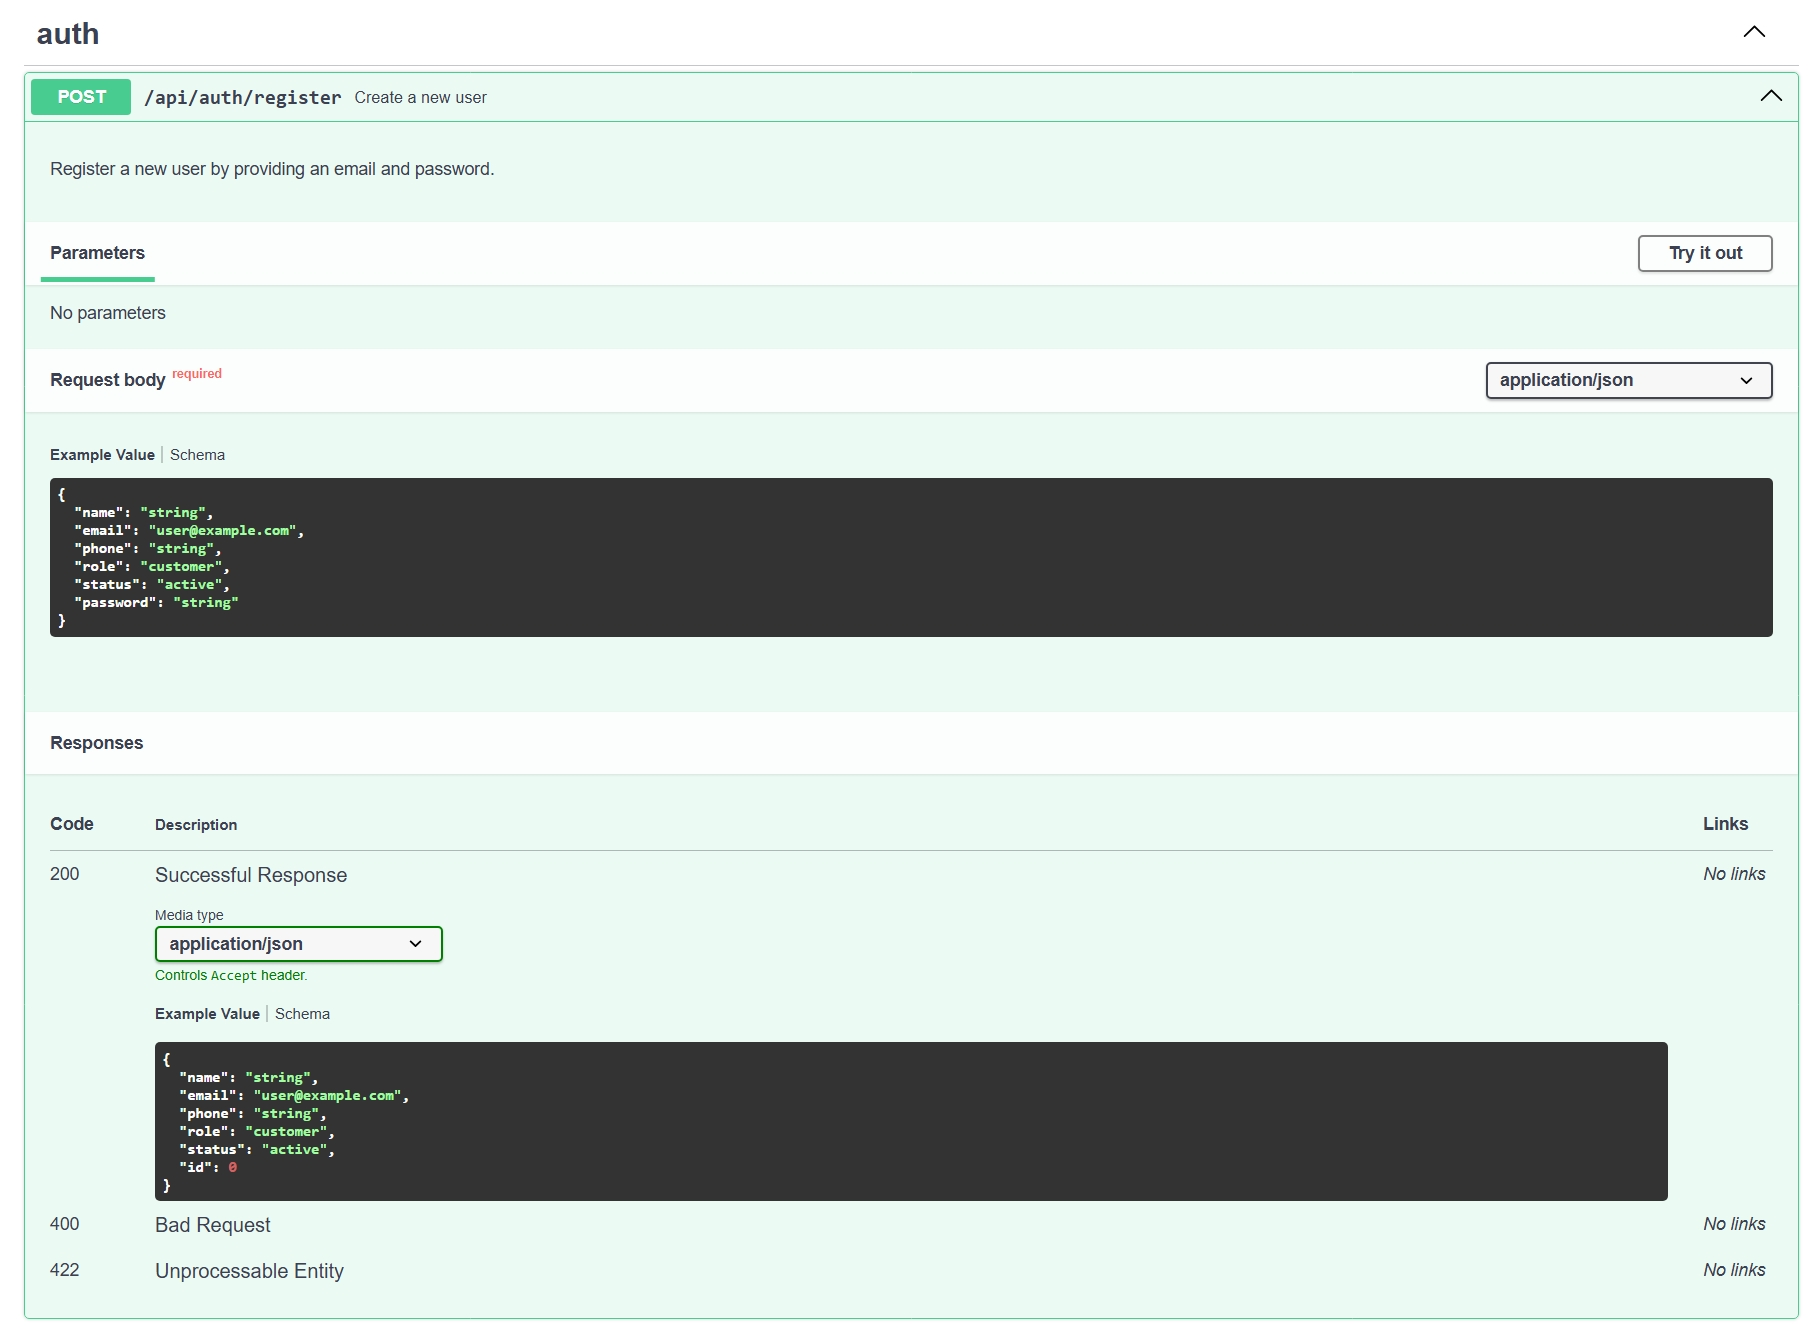
\includegraphics[width=0.96\textwidth]{API Doc - on website.jpeg}
  \caption{Embedded Swagger UI rendered inside the frontend route \apipath{/developer-apis}, including the \apipath{Authorize} control for token-based access.}
  \label{fig:frontend-swagger-authorize}
\end{figure}

\begin{figure}[H]
  \centering
  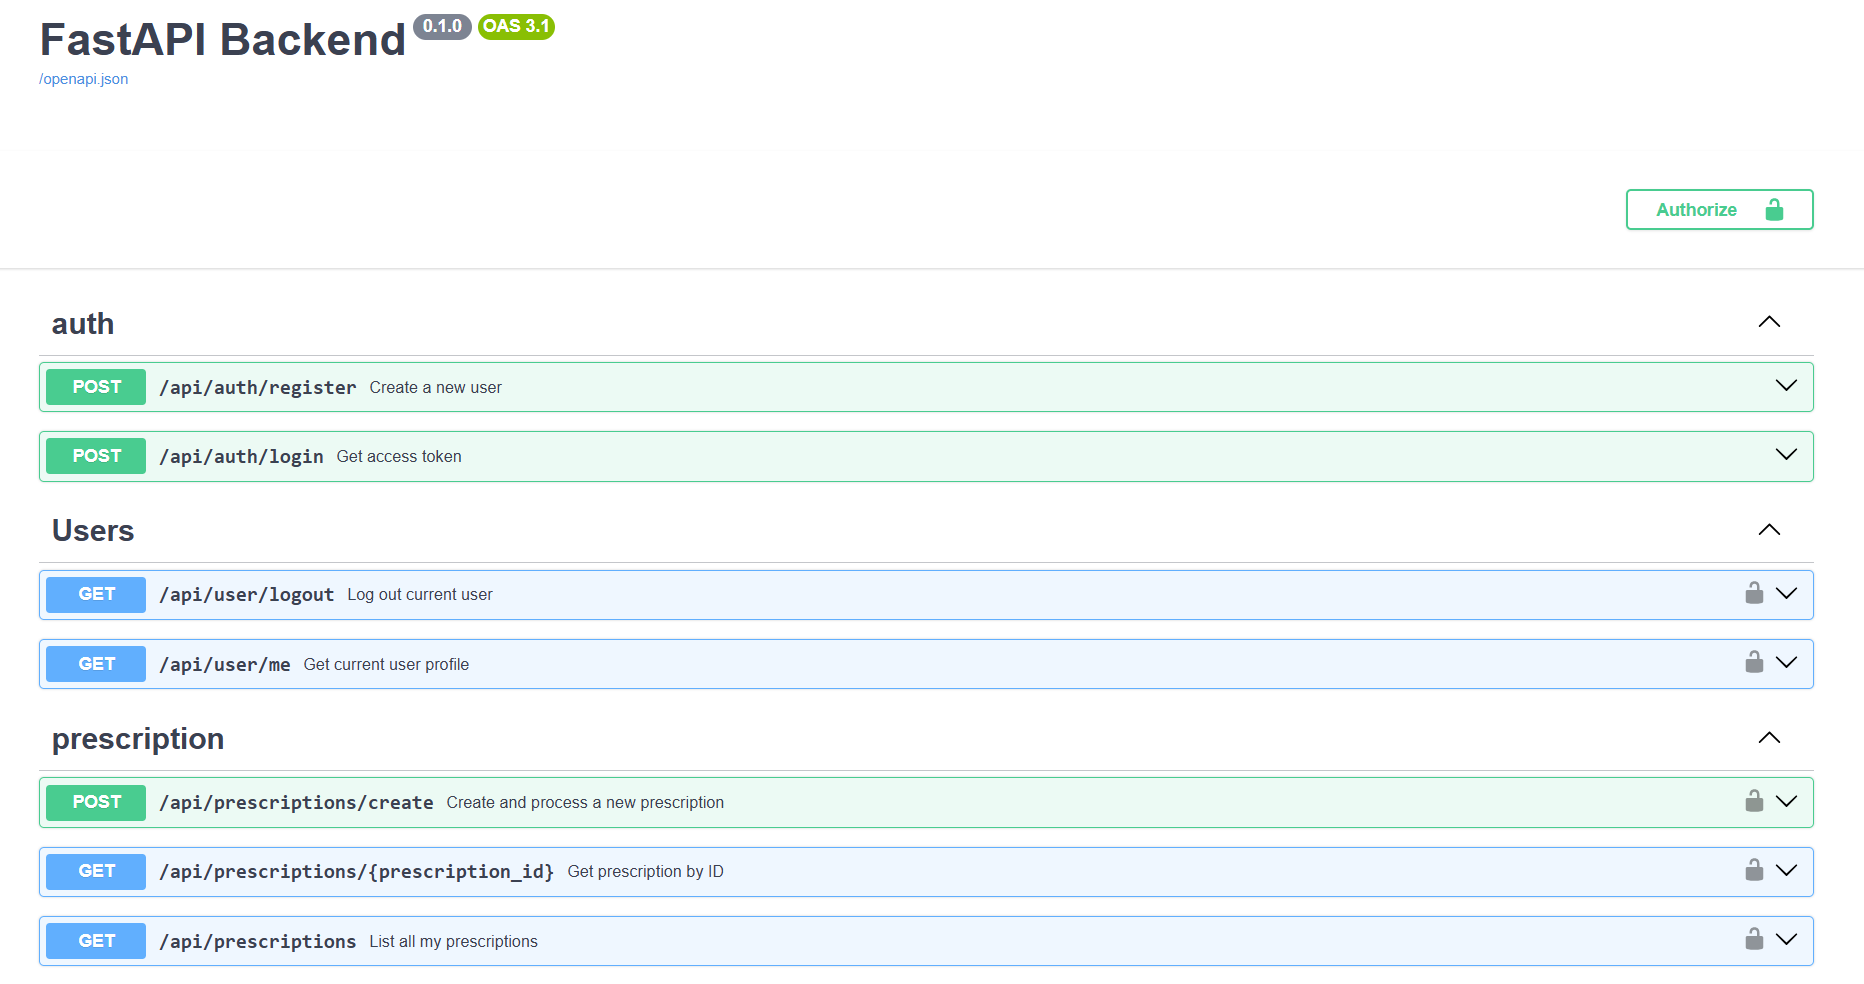
\includegraphics[width=0.96\textwidth]{API Doc Swagger.png}
  \caption{Expanded \apipath{POST /api/auth/register} endpoint view in Swagger UI showing request/response schema and execution panel.}
  \label{fig:swagger-register-endpoint}
\end{figure}

\section{API Implementations (Sprint 1)}
\subsection{Domain endpoint matrix}
\begin{longtable}{p{0.16\textwidth}p{0.18\textwidth}p{0.14\textwidth}p{0.44\textwidth}}
\toprule
\textbf{Domain} & \textbf{Router file} & \textbf{Ops count} & \textbf{Implemented endpoints} \\
\midrule
Authentication & auth_routes.py & 2 & POST \apipath{/api/auth/register}, POST \apipath{/api/auth/login} \\
User session & user_routes.py & 2 & GET \apipath{/api/user/logout}, GET \apipath{/api/user/me} \\
Doctors & doctor_routes.py & 2 & GET \apipath{/api/doctors}, GET \apipath{/api/doctors/\{doctor_id\}} \\
Appointments & appointment_routes.py & 2 & POST \apipath{/api/appointments}, GET \apipath{/api/appointments} \\
Prescriptions & prescription_routes.py & 3 & POST \apipath{/api/prescriptions/create}, GET \apipath{/api/prescriptions/\{prescription_id\}}, GET \apipath{/api/prescriptions} \\
Inventory & inventory_routes.py & 5 & GET \apipath{/api/inventory}, GET \apipath{/api/inventory/\{medicine_id\}}, POST \apipath{/api/inventory}, PUT \apipath{/api/inventory/\{medicine_id\}}, DELETE \apipath{/api/inventory/\{medicine_id\}} \\
Orders & order_routes.py & 4 & GET \apipath{/api/orders}, GET \apipath{/api/orders/\{order_id\}}, POST \apipath{/api/orders}, PUT \apipath{/api/orders/\{order_id\}} \\
Cart & cart_routes.py & 5 & GET \apipath{/api/cart}, GET \apipath{/api/cart/\{cart_item_id\}}, POST \apipath{/api/cart}, PUT \apipath{/api/cart/\{cart_item_id\}}, DELETE \apipath{/api/cart/\{cart_item_id\}} \\
Medicine requests & medicine_request_routes.py & 4 & GET \apipath{/api/medicine-requests}, GET \apipath{/api/medicine-requests/\{request_id\}}, POST \apipath{/api/medicine-requests}, PUT \apipath{/api/medicine-requests/\{request_id\}} \\
Staff & staff_routes.py & 5 & GET \apipath{/api/staff}, GET \apipath{/api/staff/\{staff_id\}}, POST \apipath{/api/staff}, PUT \apipath{/api/staff/\{staff_id\}}, DELETE \apipath{/api/staff/\{staff_id\}} \\
Customers & customer_routes.py & 3 & GET \apipath{/api/customers}, GET \apipath{/api/customers/\{customer_id\}}, PUT \apipath{/api/customers/\{customer_id\}} \\
Feedback & feedback_routes.py & 3 & GET \apipath{/api/feedback}, GET \apipath{/api/feedback/\{feedback_id\}}, POST \apipath{/api/feedback} \\
\bottomrule
\end{longtable}

\subsection{Coverage summary}
The table above maps directly to active route decorators in \apipath{backend/app/routes}. Total active operations are 40, excluding commented-out route stubs.

\section{Testing Type and Rigor}
\subsection{Type of testing used}
Sprint 1 uses API integration testing as the primary strategy through FastAPI \texttt{TestClient}. Test execution uses isolated database setup and teardown per function scope.

\subsection{Rigor and quality controls}
\begin{itemize}[leftmargin=1.2cm]
  \item Role-based request coverage for admin, employee, and customer workflows.
  \item Positive and negative scenario checks for validation, authorization, and resource updates.
  \item Isolated database lifecycle per test using fixture setup and teardown.
  \item Endpoint-level response validation on status codes and JSON payload contracts.
  \item Regression verification by running the complete backend test suite after fixes.
\end{itemize}

\subsection{Test inventory by module}
\begin{longtable}{p{0.48\textwidth}p{0.20\textwidth}p{0.22\textwidth}}
\toprule
\textbf{Test module} & \textbf{Cases} & \textbf{Focus area} \\
\midrule
\apipath{test_auth.py} & 10 & registration, login, auth validation \\
\apipath{test_cart.py} & 9 & cart CRUD and role controls \\
\apipath{test_customers.py} & 13 & customer access and updates \\
\apipath{test_feedback.py} & 14 & feedback validation and permissions \\
\apipath{test_inventory.py} & 11 & medicine CRUD and admin controls \\
\apipath{test_medicine_requests.py} & 13 & request lifecycle and role flow \\
\apipath{test_orders.py} & 13 & order creation, read, update flow \\
\apipath{test_staff.py} & 14 & staff CRUD and admin constraints \\
\midrule
\textbf{Total} & \textbf{97} & end-to-end API integration focus \\
\bottomrule
\end{longtable}

\section{Test Results}
\subsection{Automated run summary}
\begin{itemize}[leftmargin=1.2cm]
  \item Command: \apipath{pytest -q}
  \item Verification date: April 05, 2026
  \item Total tests: 97
  \item Passed: 97
  \item Failed: 0
  \item Warnings: 5
  \item Runtime: 46.53 seconds
  \item Pass rate: 100.0\%
\end{itemize}

\subsection{Representative passing test cases}
\begin{longtable}{p{0.24\textwidth}p{0.20\textwidth}p{0.20\textwidth}p{0.20\textwidth}p{0.10\textwidth}}
\toprule
\textbf{API} & \textbf{Input} & \textbf{Expected} & \textbf{Actual} & \textbf{Result} \\
\midrule
POST \apipath{/api/auth/register} & Valid user payload & 200 created user & 200 created user & \ok \\
POST \apipath{/api/auth/login} & Valid credentials & 200 token response & 200 token response & \ok \\
GET \apipath{/api/inventory} & No token & 401 unauthorized & 401 unauthorized & \ok \\
POST \apipath{/api/feedback} & Employee token & 403 forbidden & 403 forbidden & \ok \\
PUT \apipath{/api/customers/\{id\}} & Wrong customer context & 403 forbidden & 403 forbidden & \ok \\
\bottomrule
\end{longtable}

\subsection{Structured test case cards}
The following cards present representative, reviewer-friendly views of two core authentication tests from the implemented suite.

\textbf{TC-AUTH-01 --- Register Valid User}

\begin{tcolorbox}[colback=green!10,colframe=okgreen,boxrule=0.8pt,arc=2mm]
\textbf{API:} \apipath{POST /api/auth/register} \\
\textbf{Input:} \apipath{\{name, email, phone, password, role\}} \\
\textbf{Expected:} HTTP 200; response includes \apipath{id, name, email, phone, role} \\
\textbf{Actual:} HTTP 200; assertions pass for identity fields and generated \apipath{id} \\
\textbf{Result:} \passmark
\end{tcolorbox}

\textbf{TC-AUTH-02 --- Login Valid Credentials}

\begin{tcolorbox}[colback=green!10,colframe=okgreen,boxrule=0.8pt,arc=2mm]
\textbf{API:} \apipath{POST /api/auth/login} \\
\textbf{Input:} \apipath{username=customer@test.com, password=customer123} \\
\textbf{Expected:} HTTP 200; \apipath{access_token}, \apipath{token_type=bearer}, and \apipath{user} object returned \\
\textbf{Actual:} HTTP 200; JWT token emitted and user payload validated in test assertions \\
\textbf{Result:} \passmark
\end{tcolorbox}

\subsection{Pytest implementation excerpt}
Verified excerpt from \apipath{backend/tests/test_auth.py}:

\begin{lstlisting}[language=Python]
def test_register_valid_user(self, client: TestClient):
  response = client.post(
    "/api/auth/register",
    json={
      "name": "Test User",
      "email": "testuser@example.com",
      "phone": "+91-99999-99999",
      "password": "testpass123",
      "role": "customer",
    },
  )
  assert response.status_code == 200
  data = response.json()
  assert data["name"] == "Test User"
  assert data["email"] == "testuser@example.com"
  assert data["role"] == "customer"
  assert "id" in data


def test_login_valid_credentials(self, client: TestClient, customer_user):
  response = client.post(
    "/api/auth/login",
    data={"username": "customer@test.com", "password": "customer123"},
  )
  assert response.status_code == 200
  data = response.json()
  assert "access_token" in data
  assert data["token_type"] == "bearer"
  assert "user" in data
\end{lstlisting}

\subsection{Resolved failures and implemented fixes}
\begin{longtable}{p{0.30\textwidth}p{0.40\textwidth}p{0.20\textwidth}}
\toprule
\textbf{Issue} & \textbf{Fix implemented} & \textbf{Outcome} \\
\midrule
Customer self-update test mismatch & Updated \apipath{test_update_customer_self} and self-profile test to use the authenticated fixture user id rather than a newly created different customer record. & Test now passes \\
Feedback rating validation not enforced & Added request DTO \apipath{FeedbackCreate} with \apipath{rating} bounds (1..5) and switched route input to this DTO. & 422 returned for invalid ratings \\
Feedback missing comment caused DB IntegrityError & In \apipath{create_feedback}, mapped DTO to DB model and applied default comment text when omitted. & 200 response, no DB crash \\
Inventory create date type mismatch & Added \apipath{MedicineCreate} DTO and mapped payload to \apipath{Medicine} model after validation/parsing. & Date accepted, insert succeeds \\
Partial update model risks in customer/inventory update & Added \apipath{CustomerUpdate} and \apipath{MedicineUpdate} DTOs for patch-like update behavior. & Stable partial updates across tests \\
\bottomrule
\end{longtable}

\section{Documentation and Consistency Checks}
\subsection{Validated}
\begin{itemize}[leftmargin=1.2cm]
  \item \apipath{docs/openapi.yaml} exists and declares OpenAPI 3.1.0.
  \item FastAPI app exposes Swagger UI at \apipath{/docs}.
  \item FastAPI app exposes YAML at \apipath{/openapi.yaml}.
  \item Frontend app exposes embedded Swagger UI at \apipath{/developer-apis}.
  \item Embedded Swagger UI shows \apipath{Authorize} and applies token-based auth on protected operations.
\end{itemize}

\subsection{Consistency status}
\begin{itemize}[leftmargin=1.2cm]
  \item Documentation narrative is now aligned with implementation: the embedded frontend docs route exists as \apipath{/developer-apis}.
  \item Backend and frontend documentation surfaces are consistent: \apipath{/developer-apis} (frontend), \apipath{/docs} (backend Swagger), and \apipath{/openapi.yaml} (backend YAML).
\end{itemize}

\section{Action Plan for Sprint 2}
Based on verified Sprint 1 outcomes, the following actions are prioritized:

\begin{enumerate}[leftmargin=1.2cm]
  \item Reduce remaining warnings by migrating startup events to FastAPI lifespan handlers.
  \item Normalize enum serialization paths in medicine-request updates to remove serializer warnings.
  \item Add a lightweight UI smoke test for \apipath{/developer-apis} and token authorization flow in Swagger.
  \item Add CI enforcement so each merge requires full backend test pass.
\end{enumerate}

\section{User Reviews}
\subsection{Feedback collected in Sprint 1}
\begin{itemize}[leftmargin=1.2cm]
  \item Users reported that login and doctor browsing flows are clear and easy to use.
  \item Users asked for clearer error feedback when prescription extraction fails.
  \item Users requested broader admin-facing UI support for inventory and order operations.
\end{itemize}

\subsection{Action items from user feedback}
\begin{enumerate}[leftmargin=1.2cm]
  \item Improve user-facing failure messages in prescription and upload workflows.
  \item Expand frontend screens for inventory, orders, and medicine request operations.
  \item Add richer filters and paging for large API list views.
\end{enumerate}

\section{Conclusion}
Sprint 1 successfully delivered broad API coverage across all planned backend domains, with 40 active endpoints and 97 integration tests in place.

The revised report now reflects verified current-state quality rather than static assumptions. After implementing the five identified fixes (DTO-based validation for feedback and inventory, safer partial-update DTOs, and correction of self-user test targeting), the backend suite reaches 97 out of 97 passing tests.

This creates a clear, evidence-backed baseline for Sprint 2 hardening: input schema separation, stricter validation, fixture alignment, and documentation-source consistency.

\end{document}